\documentclass[xcolor=table]{beamer}

\makeatletter
\definecolor{beamer@blendedblue}{RGB}{0, 145, 95} % changed this

\usefonttheme{professionalfonts} % using non standard fonts for beamer
\usepackage{fontspec}
\setmainfont{Gill Sans}
%TIKZ

\usepackage{graphicx}
\usepackage{tikz}
\usepgflibrary{plotmarks}
\usetikzlibrary{calc,shapes.symbols,matrix,shapes.multipart,positioning,fit}
\usetikzlibrary{backgrounds}
\usetikzlibrary{decorations.pathmorphing}
\usetikzlibrary{shapes.callouts}
\usetikzlibrary{shapes.geometric}
\tikzset{snake it/.style={decorate, decoration=snake}}

% Avoid bug with callouts and Beamer, see http://tex.stackexchange.com/questions/31921/callout-and-beamer
\usetikzlibrary{decorations.text}

%for stack drawings
\usepackage{drawstack}
\usepackage{bcprules}
\usepackage{color}
\usepackage{pifont}
\usepackage{amsthm}
\usepackage{thmtools}
\usepackage{caption}
\captionsetup[figure]{labelformat=empty}

% \declaretheorem[numberwithin=chapter]{theorem}
% \declaretheorem[sibling=theorem]{definition}
% \declaretheorem[sibling=theorem]{lemma}

\usepackage{xspace}
\newcommand*{\ii}[1]{\textit{#1}}
\newcommand*{\EG}{e.g.,\xspace}
\newcommand*{\IE}{i.e.,\xspace}
\newcommand*{\ETC}{etc.\xspace}
\newcommand*{\ETAL}{{\em et al.}\xspace}
\newcommand{\atom}[2]{#1@#2}

\newcommand{\mem}[0]{\ii{mem}\xspace}
\newcommand{\imem}[0]{\ii{im}\xspace}
\newcommand{\dmem}[0]{\ii{dm}\xspace}
\newcommand{\reg}[0]{\ii{reg}\xspace}
\newcommand{\ok}[0]{\ii{ok}\xspace}
\newcommand{\acfistat}[5]{\ensuremath{(#1,#2,#3,#4,#5)}}
\newcommand{\rd}[2]{#1[#2]}
\newcommand{\upd}[3]{#1[#2{\leftarrow}#3]}
\newcommand{\pc}[0]{\ii{pc}\xspace}
\newcommand{\tpc}[0]{t_\ii{pc}}
\newcommand{\tra}[0]{t_\ii{ra}}
\newcommand{\ti}[0]{t_\ii{i}}
\newcommand{\targ}[1]{t_\ii{#1}}
\newcommand{\old}{_{\mathit{old}}}
\newcommand{\step}[2]{\ensuremath{#1\to#2}}
\newcommand{\stepn}[2]{\ensuremath{#1\to_n#2}}
\newcommand{\stepa}[3]{\ensuremath{#1\to_a^{#3}#2}}
\newcommand{\astat}[4]{\ensuremath{(#1,#2,#3,#4)}}


\newcommand{\DATA}[0]{\ii{Data}}
\newcommand{\INSTRname}[0]{\ii{Code}\xspace}
\newcommand{\INSTR}[1]{\INSTRname~#1}
\newcommand{\DATAname}[0]{\ii{Data}\xspace}
\newcommand{\CFG}[0]{$\mathcal{CFG}$\xspace}
\newcommand{\CFGm}[0]{\mathcal{CFG}\xspace}
\newcommand{\SUCC}[1]{$\mathcal{SUCC_\CFGm^{#1}}$\xspace}
\newcommand{\SUCCm}[1]{\mathcal{SUCC_\CFGm^{#1}}\xspace}

\newcommand{\frule}[8]{#1:\{\ifthenelse{\equal{#2}{}}{}{\mathit{PC}{=}#2\ifthenelse{\equal{#3}{}}{}{,}}
                           \ifthenelse{\equal{#3}{}}{}{\mathit{CI}{=}#3}\ifthenelse{\equal{#4}{}}{}{,}
                           \ifthenelse{\equal{#4}{}}{}{\mathit{OP}_1{=}#4}\ifthenelse{\equal{#5}{}}{}{,}
                           \ifthenelse{\equal{#5}{}}{}{\mathit{OP}_2{=}#5}\ifthenelse{\equal{#6}{}}{}{,}
                           \ifthenelse{\equal{#6}{}}{}{\mathit{MR}{=}#6}
                           \} \to \{\mathit{PC}'{=}#7, \mathit{RES}{=}#8\}}

\newcommand{\TAGS}[1]{$\mathcal{T} = \lbrace #1 \rbrace$}

\definecolor{ForestGreen}{RGB}{0, 155, 85}
\definecolor{Purple}{RGB}{153, 71, 155}
\definecolor{BrickRed}{RGB}{182, 50, 28}
\definecolor{darkgreen}{cmyk}{0.7, 0, 1, 0.5}

\begin{document}
\title{Formally Verified Tag-Based Enforcement of Control Flow Integrity}   
\author{Nick Giannarakis} 
\date{\today} 

\pgfdeclarelayer{background}
\pgfdeclarelayer{foreground}
\pgfsetlayers{background,main,foreground}

\frame{\titlepage} 

\frame{
 \begin{itemize}
   \item Slide 1, attacks that attempt to circumvent the control-flow.
                 diagram
         Slide 2,
         Effective mitigation technique called CFI
   \item Slide 3, Micro-policies tag data with meta-data, software rules on meta-data
                 Efficient implementation with hardware propagation of metadata and rule cache, policy monitor
         Slide 4, Micro-policies framework modelling PUMP. Symbolic machine abstracting away from low-level details        
    \item Slide 5,6 Fine-grained CFI micro-policy
      \item Slide 7, Formal verification of CFI outline, proof of CFI property for concrete machine, refinement between
        abstract machine and concrete
        Slide 8, Abstract machine
        Slide 9, Symbolic machine as an intermediate step (a few slides adding stuff on the go) to two-way refinement.
                 leverage micro-policies framework to get concrete-symbolic refinement
        Slide 10, Property characterizing CFI
        Slide 16, Proof Technique
        Slide 11, Generic CFI machine
        Slide 12-13, Examples instantiation abstract machine, proof for abstract machine
        Slide 14-15, Generic Preservation Theorem
        Slide 16, Symbolic instance of CFI machine
        Slide 17-18, Symbolic-Abstract preservation
        Slide 19, Concrete instance
        Slide 20-21, Concrete-Symbolic preservation
        Slide 22, Conclusions, future work, etc.
      \end{itemize}
}

%1st run : 70sec
\frame{
\frametitle{Motivation}
Modern computers are vulnerable to a wide-range of attacks.
\begin{block}{Common Attack techniques}
\begin{itemize}
\item Hijack the control-flow of the program to direct execution to
attacker code
\item Usually achieved by exploiting low-level vulnerabilities, \EG buffer overflows.
\end{itemize}
\end{block}
\begin{block}{Mitigation techniques}
  \begin{itemize}
  \item Mostly low-level ad-hoc solutions (\EG ASLR, stack canaries, \ETC)
  \item Only make it harder to exploit vulnerabilities
  \item Lack (formal) reasoning about class of attacks thwarted 
  \end{itemize}
\end{block}
% \centering
% \begin{minipage}[b]{0.2\linewidth}
% \centering
% \tikzstyle{attackercell}=[fill=red!30,draw=black,font=\tiny]
%  \begin{drawstack}[scale=0.5,font=\tiny]
%   \cell[attackercell]{Attacker Code}
%   \padding{3}{Unallocated Stack}
%   \cell{char *buffer} \cellptr{SP}
%   \cell{Return Address}
% \end{drawstack}
% \end{minipage}
% \hspace{0.5cm}
% \begin{minipage}[b]{0.25\linewidth}
% \centering
% \tikzstyle{attackercell}=[fill=red!30,draw=black,font=\tiny]
%  \begin{drawstack}[scale=0.5,font=\tiny]
%   \cell[attackercell]{Attacker Code}
%   \padding{3}{Unallocated Stack}
%   \cell[attackercell]{char *buffer}
%   \cell[attackercell]{Return Address} 
%   \cellround{Now points to Attacker Code}
% \end{drawstack}
% \end{minipage}
}

%1st run: 53sec
\frame{
\frametitle{Control-Flow Integrity}
Constraints all execution paths to follow a statically computed control-flow graph.
\begin{itemize} 
\item Formally provable that CFI defends against attackers who have control over the memory and registers of the machine
  \begin{itemize}
    \item Buffer overflows
    \item Jump-to-libc
    \item Pointer subterfuge
    \end{itemize}
\item Effectiveness (and efficiency) determined by precision of the CFG.
  \begin{itemize}
    \item \textit{Coarse-grained} CFI uses a conservative CFG 
      (\EG instructions are either jump targets or not)
    \end{itemize} 
\item Well studied defense technique
  \begin{itemize}
    \item Original CFI for x86 plus formal (but not machine-checked) study by Abadi \ETAL
    \item More efficient implementation by Zhang \ETAL
    \item Attacks on coarse-grained CFI by G{\"o}tkas \ETAL
    \end{itemize}
\end{itemize}
}

%50 sec
\frame{ 
\frametitle{Contributions} 
  Formalized and verified, using the
  Coq proof assistant, a dynamic monitor for CFI, based on a generic
  hardware-software mechanism.
\begin{itemize} 
\item Provided precise attacker model and proved that execution follows the control-graph even in the presence of an attacker (variant of Abadi \ETAL property) \pause
\item Proved a two-way refinement between the concrete machine running
  the CFI dynamic monitor and an abstract machine that has CFI by
  construction \pause
\end{itemize}
\textbf{Challenge:} Avoid direct proof of CFI property on concrete machine
}

\frame{
\frametitle{Micro-policies}
\begin{block}{Key Ideas}
  \begin{itemize}
  \setlength{\itemsep}{1pt}
    \item Associate meta-data (tags) to each machine word
    \item Use rules to check invariants on meta-data and propagate them
  \end{itemize}
\end{block}\pause

\begin{block}{Efficient hardware-software implementation}
\begin{itemize}
  \setlength{\itemsep}{1pt}
  \item Hardware propagates the meta-data according to software rules (policy monitor)
  \item Hardware rule cache for common-case efficiency
\end{itemize}
\end{block}\pause

\begin{block}{Verification framework}
\begin{itemize}
  \setlength{\itemsep}{1pt}
  \item Models hardware-software mechanism from above
  \item Intermediate step (Symbolic machine) abstracts away from low-level hardware details
  \item $\lbrace 0,1 \rbrace$-backward simulation between Concrete and Symbolic
\end{itemize}
\end{block}
}

\frame{
\frametitle{CFI Micro-policy}
Build on top of non-writable code (NWC) and non-executable data (NXD) micro-policy.
\begin{block}{Set of tags}
  \TAGS{\DATA,\INSTR{\ii{id}}, \INSTR{\bot}}
\end{block}
\begin{block}{Initial tagging scheme}
  \begin{itemize}
  \item Sources/targets of indirect control-flows (according to CFG) tagged using their address (\textit{addr})
    \INSTR{\textit{addr}}
  \item All other instructions tagged $\INSTR{\bot}$
  \item Non-executable data tagged \DATA.
  \end{itemize}
\end{block}
}

\frame{
\frametitle{CFI micro-policy}
\framesubtitle{Example}
\begin{table}[h]
\centering
\small
\begin{tabular}{lllcll}
                          &              &             & r                                                &           &           \\ \cline{2-6} 
\multicolumn{1}{c|}{Regs} & \multicolumn{2}{c|}{$\ldots$} & \multicolumn{1}{c|}{\atom{500}{\DATA}} & \multicolumn{2}{l|}{$\ldots$} \\ \cline{2-6} 
\end{tabular}
\end{table}

\centering
\begin{minipage}[b]{0.42\linewidth}
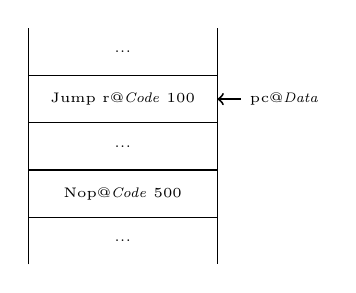
\begin{tikzpicture}[scale=0.6,font=\tiny]
  \small
  \stacktop[]{}
  \cell[]{\atom{Jump r}{\INSTR{100}}} \celladdr{100} \cellptr{\atom{pc}{\DATA}}
  \stackbottom[]{}
  \cell[]{\atom{Nop}{\INSTR{500}}} \celladdr{500}
  \stackbottom[]{}
\end{tikzpicture}
\end{minipage}
\hspace{0.5em}
\begin{minipage}[b]{0.45\linewidth}
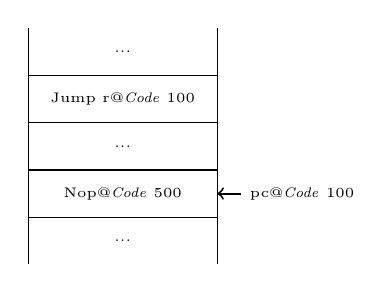
\begin{tikzpicture}[scale=0.6,font=\tiny]
  \small
  \stacktop[]{}
  \cell[]{\atom{Jump r}{\INSTR{100}}} \celladdr{100} 
  \stackbottom[]{}
  \cell[]{\atom{Nop}{\INSTR{500}}} \celladdr{500} \cellptr{\atom{pc}{\INSTR{100}}}
  \stackbottom[]{}
\end{tikzpicture}
\end{minipage}
$(100,500) \in \CFGm$?
}

\frame{
\frametitle{CFI Micro-Policy}
\framesubtitle{Rules}
% \def\beforelabelspacehack{\vspace*{-2ex}}
\small
\infrule[]{
  \ii{op} \in \lbrace \ii{Jump}, \ii{Jal} \rbrace \andalso
  (src,dst) \in \CFGm
  }{
  \ii{op} : \{PC=\INSTR{src},CI=\INSTR{dst}\} \to (\INSTR{dst},-)
  }
\infrule[]{
  \ii{op} \in \lbrace \ii{Jump}, \ii{Jal} \rbrace
  }{
    \ii{op} : \{PC=\DATA,CI=\INSTR{\textit{src}}\} \to (\INSTR{src},-)
  }
\infrule[]{
  (src,dst) \in \CFGm
  }{
  \ii{Store} : \{PC=\INSTR{src},CI=\INSTR{dst},MR=\DATA\} \to (\DATA,\DATA)}
\infrule[]{
  \textit{ti} \in \lbrace \INSTR{dst}, \INSTR{\bot} \rbrace
  }{
  \ii{Store} : \{PC=\DATA,CI=\textit{ti},MR=\DATA\} \to (\DATA,\DATA)
  }
\infrule[]{
  \textit{op} \not \in \lbrace \textit{Jump}, \textit{Jal}, \textit{Store}
  \rbrace \andalso (src,dst) \in \CFGm
  }{
  \textit{op} : \{PC=\INSTR{src},CI=\INSTR{dst}\} \to (\DATA,-)
  }
\infrule[]{
  \textit{op} \not \in \lbrace \textit{Jump}, \textit{Jal}, \textit{Store}
  \rbrace \andalso
  \textit{ti} \in \lbrace \INSTR{dst}, \INSTR{\bot} \rbrace
  }{
  \textit{op} :\{PC=\DATA,CI=\textit{ti}\} \to (\DATA,-)
  }
}

%Symbolic Machine
\begin{frame}[fragile]
\frametitle{CFI Symbolic Machine}
\begin{itemize}
\item Uses tags mentioned above
\item \textit{transfer} function that implements the rules for CFI
\end{itemize}
\infrule[Jump]{
  \mem[\pc] = \atom{i}{t_i} \andalso \ii{decode}~i = \ii{Jump}~r \\
  \rd{\reg}{r} = \atom{\pc'}{t_w} \andalso
  \ii{transfer}~(t_{pc},t_i,t_w,-,-) = (t_{pc}',-)
  }{\step{\astat{\mem}{\reg}{\atom{\pc}{t_{pc}}}{int}}
  {\astat{\mem}{\reg}{\atom{w}{t_{pc}'}}{int}} }
\end{frame}

%Concrete Machine
\begin{frame}
\frametitle{CFI Concrete Machine}
\begin{itemize}
\item Wraps symbolic tags around tags of self-protection mechanism
  \begin{itemize}
    \item \textit{User ut} where $ut \in \mathcal{T}$
    \item \textit{Monitor} for policy-monitor data
    \item \textit{Entry ut} for calling privileged monitor services from user code
    \item We provide encoding function from (wrapped) tags to machine words
    \end{itemize}
\item \textit{Policy monitor} is a \emph{correct} implementation of the transfer function in machine code
\end{itemize}
\end{frame}

%Abstract Machine
\frame{
\frametitle{CFI Abstract Machine}
The Abstract Machine acts as a specification for CFI
\begin{itemize}
\item Instructions fetched from fixed instruction memory (NWC, NXD)
\item State includes \ok bit as indication of a violation. The machine is stuck if it is set to false.
\end{itemize}
\infrule[Jump]{
  \imem[\pc] = i \andalso \ii{decode}~i = \ii{Jump}~r \\
  \rd{\reg}{r} = \pc' \andalso
  \ii{ok} = (\pc,\pc') \in \CFGm
  }{\step{\acfistat{\imem}{\dmem}{\reg}{\pc}{\ii{true}}}{
    \acfistat{\imem}{\dmem}{\reg'}{\pc'}{\ii{ok}}}}
}

\frame{
\frametitle{Attacker Model}
\begin{block}{Intuition}
  \begin{itemize}
  \item Can change all (user-level) data in memory and registers
  \item But \textbf{not} the code or the tags for tagged machines
  \end{itemize}
\end{block}
\begin{block}{Formally}
  \infrule{
  \ii{dom}~\dmem = \ii{dom}~\dmem' \andalso
  \ii{dom}~\reg = \ii{dom}~\reg'
}{
  \stepa{\acfistat{\imem}{\dmem}{\reg}{\pc}{\ok}}
  {\acfistat{\imem}{\dmem'}{\reg'}{\pc}{\ok}}
  {A}}
  \infrule[]{
  }{\stepa{\atom{w_1}{\DATA}}{\atom{w_2}{\DATA}}{S}}
  \infrule[]{
  }{\stepa{\atom{w_1}{\INSTR{id}}}{\atom{w_1}{\INSTR{id}}}{S}}
\end{block}
}

\frame{
\frametitle{CFI Property}
\begin{block}{Definition parameterized by:}
  \begin{itemize}
    \item Set of states \textit{S}
    \item \textit{Initial} states predicate
    \item Attacker model
    \item \emph{Extended} CFG to direct control-flow \SUCC{}
    \item \textit{Stopping} predicate characterizing execution after a control-flow violation
  \end{itemize}
  $$M=(\textit{S},\textit{initial},\stepn{}{},\stepa{}{}{},\SUCCm{},\textit{stopping})$$
\end{block}
}

\frame{
\frametitle{CFI Property}
\framesubtitle{Definitions}
\begin{definition}[Trace has CFI]\label{traceHasCfi}
  We say that an execution trace $s_0 \to s_1 \to \ldots \to s_n$ {\em has CFI}
  if for all $ i \in [0,n)$ if \stepn{s_i}{s_{i+1}} then
  $(s_i,s_{i+1}) \in$ \SUCC{}.
\end{definition}\pause
\vspace*{0em}
\begin{alertblock}{
More complex than Abadi \ETAL because our mechanism detects a violation one step later!}
\end{alertblock}
\vspace*{-1.4em}
\begin{definition}[CFI]\label{cfi}
  A CFI machine M has CFI with respect to the set of allowed indirect jumps \CFG
  if, for any execution starting from initial state $s_0$
  and producing a trace $s_0 \to \ldots \to s_n$, either
  \begin{enumerate}
  \setlength{\itemsep}{1pt}
  \item The whole trace \emph{has CFI} according to
    the above definition, or else
  \item There is some $i$ such that $s_i \to_n s_{i+1}$,
  and $(s_i, s_{i+1}) \not \in$ \SUCC{}, where
  the sub-traces $s_0 \to \ldots \to s_i$ and
  $s_{i+1} \to \ldots \to s_n$ both have CFI
  and the sub-trace $s_{i+1} \to \ldots \to s_n$ is stopping.
  \end{enumerate}
\end{definition}
}

\frame{
\frametitle{CFI Property}
\framesubtitle{Instances of definitions I}
\begin{block}{Abstract Machine}
  \begin{itemize}
    \setlength{\itemsep}{1pt}
    \item $\mathit{initial^A}$ : \ok bit set to true
    \item \SUCC{A} : Extends \CFG with direct control-flows (\EG Nop targets pc+1)
    \item $\mathit{stopping^A}$ : All states in trace are stuck with respect to \stepn{}{}
  \end{itemize}
\end{block}

\begin{block}{Symbolic Machine}
  \begin{itemize}
    \setlength{\itemsep}{1pt}
    \item $\mathit{initial^S}$ : Indirect jumps and their targets tagged according to \CFG (invariant and tag on PC is \DATA.
    \item \SUCC{S} : Extends \CFG with direct control-flows (\EG Nop targets pc+1)
    \item $\mathit{stopping^S}$ : All states in trace are stuck with respect to \stepn{}{}
  \end{itemize}
\end{block}
}

\frame{
\frametitle{CFI Property}
\framesubtitle{Instances of definitions II}
\begin{block}{Concrete Machine}
  \begin{itemize}
    \setlength{\itemsep}{1pt}
    \item $\mathit{initial^C}$ : Image of a symbolic state $s^S$ such that $s^S \sim s^C$
    \item \SUCC{C} : Extends \CFG with direct-flows, allows all flows involving monitor mode
    \item $\mathit{stopping^C}$ : There is an optional prefix of attacker steps followed by an optional suffix of
      monitor (normal) steps
  \end{itemize}
\begin{center}
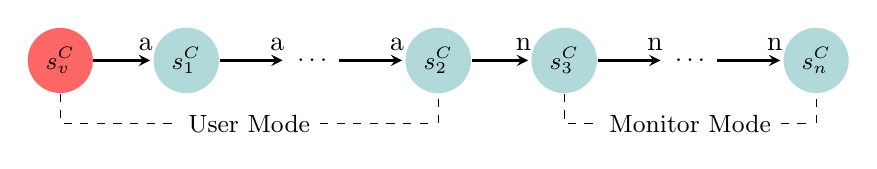
\begin{tikzpicture}
  [scale=.8,auto=left,shorten >=1pt,every node/.style={circle,fill=teal!30,font=\small},->,>=stealth]
  \node (nv) [style={fill=red!60}] at (0,0)  {$s^C_v$};
  \node (na1) at (2,0)  {$s^C_1$};
  \node (nadots) [draw=none,style={fill=white}] at (4,0)  {$\ldots$};
  \node (na2) at (6,0)  {$s^C_2$};
  \node (nm1) at (8,0)  {$s^C_3$};
  \node (nmdots) [draw=none,style={fill=white}] at (10,0)  {$\ldots$};
  \node (nm2) at (12,0)  {$s^C_n$};

\node (nulabel) [rectangle,fill=white,font=\small] at (3,-1) {User Mode};
\node (na2label) [fill=none] at (6,-1) {};

\node (nmlabel) [rectangle,fill=white,font=\small] at (10,-1) {Monitor Mode};
\node (nm2label) [fill=none] at (12,-1) {};

\draw[-,dashed,very thin] (nv) |- (nulabel);
\draw[-,dashed,very thin] (nulabel.east) |- (na2label.center);
\draw[-,dashed,very thin] (na2label.center) |- (na2.south);

\draw[-,dashed,very thin] (nm1) |- (nmlabel);
\draw[-,dashed,very thin] (nmlabel.east) |- (nm2label.center);
\draw[-,dashed,very thin] (nm2label.center) |- (nm2.south);

\path[thick, every node/.style={}]
(nv) edge [very near end,above] node {a} (na1)
(na1) edge [very near end,above] node {a} (nadots)
(nadots) edge [very near end,above] node {a} (na2)
(na2) edge [very near end,above] node {n} (nm1)
(nm1) edge [very near end,above] node {n} (nmdots)
(nmdots) edge [very near end,above] node {n} (nm2);
\end{tikzpicture} \\
\end{center}
\end{block}
}

\frame{
\frametitle{CFI Micro-Policy Verification}
  \begin{center}
    \begin{tikzpicture}
      [machine/.style={rectangle,draw=teal!80,fill=teal!10,text=black,very thick,minimum height=1cm},
       cfi/.style={rectangle,draw,thick,draw=teal!80,text=black,fill=teal!10},
       >=stealth]

      % abstract
      \onslide<3->{\node [machine,fill=teal!10] (abstract) {Abstract Machine};}

      % symbolic-rule
      \node (symbolic label) [below=2.5cm of abstract] {Symbolic Machine};
      \node [rectangle,draw,thick,fill=teal!20,rounded corners]
            (symbolic rules) [right=of symbolic label] {CFI Micro-Policy};
      \begin{pgfonlayer}{background}
        \node [machine,dashed,fill=teal!10,fit={(symbolic label) (symbolic rules)}]
              (symbolic) {};
      \end{pgfonlayer}
      \onslide<5->{\node [cfi,right=of symbolic] (symbolic cfi) {CFI Property};}

      %abstract cfi
      \onslide<4->
      {\node [cfi] (abstract cfi)  at (abstract -| symbolic cfi) {CFI Property};
       \draw [thick] (abstract) to (abstract cfi);}

      %symbolic cfi
      \onslide<5->{
        \draw [thick] (symbolic) to (symbolic cfi);
        \draw [->,thick]
              (abstract cfi)
              to node [right] {Preserved}
              (symbolic cfi);}

      % concrete
      \onslide<2->{\node (concrete label) [below=2.5cm of symbolic label] {Concrete
        Machine};
      \node [rectangle,draw,thick,fill=red!30,rounded corners]
            (fault handler) [right=of concrete label] {CFI Policy Monitor};
      \begin{pgfonlayer}{background}
        \onslide<2->{
        \node [machine,dashed,fill=teal!10,fit={(concrete label) (fault handler)}]
              (concrete) {};}
      \end{pgfonlayer}}
      % \draw [thick,dashed] (concrete) to (concrete cfi);
      \onslide<6->{\node [cfi] (concrete cfi) at (concrete -| symbolic cfi) {CFI Property};}


      \onslide<2->{\draw [color=red!80,thick,->]
        (symbolic rules.center |- symbolic rules.south)
        -- node [right] {Compiled to}
        (symbolic rules.center |- fault handler.north);}

      \onslide<2->{\draw [<->,thick,dashed]
            (abstract.center |- symbolic.south)
            -- node [left] {Simulates}
            (abstract.center |- concrete.north);}

      \onslide<3->{\draw [<->,thick]
            (abstract)
            -- node [left] {Simulates}
            (abstract.center |- symbolic.north);}

       \onslide<6-> {
         \node [color=ForestGreen,scale=1.4] (success) [right=0.1cm of concrete cfi] {\ding{51}};
         \draw [thick] (concrete) to (concrete cfi);
         \draw [->,thick]
              (symbolic cfi)
              to[] node [right] {Preserved}
              (concrete cfi);}
    \end{tikzpicture}
  \end{center}
}

\frame{
\frametitle{Generic Preservation Theorem}
\framesubtitle{Requirements}
\textbf{Backward simulation preserves CFI}
\begin{itemize}
  \setlength{\itemsep}{1pt}
  \item High-level machine $M^H$ related to low-level machine $M^L$ by simulation relation $\sim$
  \item Predicate \textit{checked} on low-level normal steps indicates if step must be checked for CFI 
  \item $\lbrace 0,1 \rbrace$-backward simulation for unchecked steps
  \item 1-backward simulation for checked and attacker steps \pause
  \item Plus additional assumptions: 
    \begin{itemize}
      \item On initial states, low-level initial states can be mapped to high-level initial states
      \item On successor functions, for checked steps \SUCC{H} and \SUCC{L} agree on their results
        and for unchecked steps \SUCC{L} allows all steps
      \item On normal steps that are violations, we require that they cannot be attacker steps as well
      \item On stopping traces, a high-level stopping trace is simulated only by a low-level stopping trace
      \end{itemize}
\end{itemize}
}

\frame{
\frametitle{Using the Preservation Theorem}
\begin{block}{Symbolic-Abstract}
\begin{itemize}
  \item All steps are checked
  \item We have proved 1-backward simulation for normal and attacker steps.
\end{itemize}
\end{block}

\begin{block}{Concrete-Symbolic}
\begin{itemize}
  \item Steps involving the monitor are unchecked
    \begin{itemize}
      \item But by definition of \SUCC{C} they are allowed
      \end{itemize}
  \item We can obtain a $\lbrace 0,1 \rbrace$-backward simulation for normal steps from the framework.
  \item We prove 1-backward simulation for attacker steps.
\end{itemize}
\end{block}
}

\frame{
\frametitle{Future Work}
\begin{itemize}
\item Write and verify the machine code for the monitor
  \begin{itemize}
    \item More interesting for more realistic RISC architectures (\EG ARM)
    \item Could also test the code (using QuickChick!) - requires CFG
    \end{itemize}
\item Increase precision by enforcing call-stack protection to ensure correct returns
\end{itemize}
}

% \begin{frame}[fragile]
% \begin{minipage}{\linewidth}
%   \centering
%   \begin{minipage}{0.45\linewidth}
%     \begin{figure}[H]
%       \begin{center}
%         \begin{tikzpicture}
%           \matrix (m) [matrix of math nodes,row sep=3em,column sep=4em,minimum width=2em]
%           {
%             s^L_1 & s^L_2 \\
%         s^H_1 & s^H_2 \\};
%       \path[->]
%       (m-1-1) edge [snake it,-] node {} (m-2-1)
%       edge [above] node [above,very near end,font=\small] {n} (m-1-2)
%       (m-2-1.east|-m-2-2) edge [dashed, above,very near end,font=\small] node {n}
%       node {} (m-2-2)
%       (m-1-2) edge [snake it,dashed,-] node {} (m-2-2);
%     \end{tikzpicture}
%        \end{center}
%        \caption{1-backward simulation}
%      \end{figure}
%   \end{minipage}
%   \hspace{0.05\linewidth}
%   \begin{minipage}{0.45\linewidth}
%     \begin{figure}[H]
%       \begin{center}
%         \begin{tikzpicture}
%           \matrix (m) [matrix of math nodes,row sep=3em,column sep=4em,minimum width=2em]
%           {
%             s^L_0 & s^L_1 \\
%             s^H\\};
%           \path[->]
%           (m-1-1) edge [snake it,-,above] node {} (m-2-1)
%           (m-1-1.east|-m-1-2) edge [above,font=\small, very near end] node {n}
%           node {} (m-1-2)
%           (m-1-2) edge [snake it,dashed,-] node {} (m-2-1);
%         \end{tikzpicture}
%       \end{center}
%       \caption{0-backward simulation}
%     \end{figure}
%   \end{minipage}
% \hspace{0.05\linewidth}
%   \begin{minipage}{0.45\linewidth}
%     \begin{figure}[H]
%       \begin{center}
%         \begin{tikzpicture}
%           \matrix (m) [matrix of math nodes,row sep=3em,column sep=4em,minimum width=2em]
%           {
%             s^L_1 & s^L_2 \\
%             s^H_1 & s^H_2 \\};
%           \path[->]
%           (m-1-1) edge [snake it,-] node {} (m-2-1)
%           edge [above] node [above,very near end,font=\small] {a} (m-1-2)
%           (m-2-1.east|-m-2-2) edge [dashed, above,very near end,font=\small] node {a}
%           node {} (m-2-2)
%           (m-1-2) edge [snake it,dashed,-] node {} (m-2-2);
%         \end{tikzpicture}
%       \end{center}
%       \caption{1-backward simulation for attacker}
%     \end{figure}
%     \bigskip
%   \end{minipage}
% \end{minipage}
% \end{frame}
\end{document}

